%! TEX root = **/010-main.tex
% vim: spell spelllang=en:

\subsection{Na\"ive Bayes}%
\label{sub:naive-bayes}

\newcommand{\sresults}[2]{
\begin{table}[H]
\centering
\begin{tabular}{lc}
Confusion matrix on test set: & \( \begin{bmatrix} #1 \end{bmatrix} \) \\
    \addlinespace[0.5em]
    Accuracy on test set: & #2
\end{tabular}
\end{table}
}

\newcommand{\fresults}[3]{
\begin{table}[H]
\centering
\begin{tabular}{lc}
Confusion matrix on test set: & \( \begin{bmatrix} #1 \end{bmatrix} \) \\
    \addlinespace[0.5em]
    Accuracy on test set: & #2 \\
    F1 score on test set: & #3
\end{tabular}
\end{table}
}

% Think about hypothesis of independence of variables.  Do you have enough number of elements to obtain reliable probabilities?
% Keep that information for the discussion section.


Na\"ive Bayes works on the assumption of independence between variables in the dataset. First of all we checked weather or not 
this is a reasonable assumption in our dataset. To do so we calculated the correlation matrix, the farther apart the correlations 
are from 0 the more dependence there is between variables.

% Add correlation Matrix image

As we see in \cref{corr_mat} despite seeing some strong correlations between pairs of variables, for most pairs these values are much closer to 0 than expected. 
Therefore it isn't that far-fetched to assume independence between variables.

There are several types of Na\"ive Bayes algorithms:
\begin{itemize}[topsep=0pt]
    \item Gaussian NB: Used when feature space is quantitative
    \item Bernoulli NB: Used when feature space is Binary
    \item Multinomial NB: Used when feature space is discrete counts
\end{itemize}

Our data consists mostly of numerical quantitative variables, therefore Gaussian Na\"ive Bayes will be applied from here on.

\subsection{Normalization}

We executed the algorithm with no preprocessing, with standardization (mean=0, std=1) and we also tried Power Transform, which is an algorithm that tries to make our data more Gaussian-like.

\begin{table}[H]
\centering
\begin{tabular}{lccc}
\toprule
    & No normalization & Standardization & Power Transform \\
    \midrule
    Confusion matrix & 
    \( \begin{bmatrix} 208 & 200 \\ 3 & 189 \end{bmatrix} \) & 
    \( \begin{bmatrix} 287 & 121 \\ 2 & 190\end{bmatrix} \) &
    \( \begin{bmatrix} 357 & 51 \\ 19 & 173\end{bmatrix} \)
    \\
    \addlinespace[0.5em]
    Accuracy: & 0.661 & 0.795 & 0.883 \\
    F1 score: & 0.65 & 0.755 & 0.831 \\
    \bottomrule
\end{tabular}
\end{table}


One of the problems we had when performing Na\"ive Bayes is that most of our data are continuous variables
which don't exactly follow a normal distribution. Gaussian Na\"ive Bayes will treat out data as if they followed 
a Gaussian distribution. That is why the f1-score and accuracy of the Power transformed data is much better than the 
others.

\subsection{Parameter tuning}

Na\"ive Bayes doesn't have many hyperparameters, in fact we will only analyse \texttt{var\_smoothing} which determines the amount Laplace smoothing applied.

\begin{figure}[H]
    \centering
    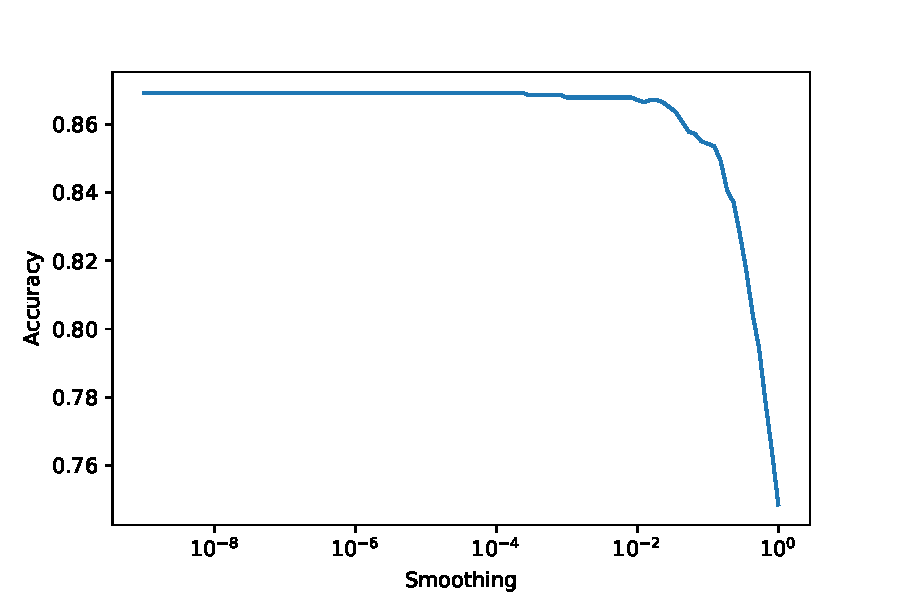
\includegraphics{figures/naive_bayes_smoothing_cv.pdf}
    \caption{Na\"ive Bayes smoothing}%
    \label{fig:naive_bayes_smoothing_cv}
\end{figure}

Looking at the image we can see that the f1-score barely changes when the \texttt{var\_smoothing} is in the range $[10^{-9}, 10^{-2}]$. Therefore its better to leave the default $10^{-9}$.
